\documentclass[a4paper]{article}

\usepackage{amsmath}
\usepackage{amssymb}
\usepackage{stellar}
\usepackage{parskip}
\usepackage{fullpage}
\usepackage{wrapfig}
\usepackage{tikz}

\title{Probability}
\author{Paolo Bettelini}
\date{}

\begin{document}

\maketitle
\tableofcontents

\section{Probabilità}

\subsection{Costruzione intuitiva}

\sexample{Approccio classico alla probabilità}{
    Consideriamo un'urna contenente 6 palline numerate da \(1\) a \(6\) e per il resto indistinguibili.
    Vogliamo studiare l'esperimento estrazione di una pallina dall'urna.
    Voglio studiare quale pallina sia più probabile che venga estratta.
    Vogliamo quindi mettere un ordinamento sull'insieme degli eventi di questo esperimento.
    Sia \(\Omega\) l'insieme di tutti i possibili risultati dell'esperimento.
    Sia \(P_i\) la probabilità di estrarre il numero \(i \in \{1,2,3,5,6\}\).
    In questo caso la scelta naturale è \(P_i = \frac16\) per tutte le \(i \in \{1,2,3,4,5,6\}\).
    Notiamo che \(\sum P_i = 1\), cioè la probabilità di estrarre un numero da \(1\) a \(6\), cioè in questo
    caso l'evento certo. Questa viene detta additività della probabilità di eventi disgiunti.
    Inoltre, la probabilità \(P_j = 0\) con \(j \notin \{1,2,3,4,5,6\}\).
    Possiamo anche notare che
    \[
        P_i = \frac{\text{Casi favorevoli}}{\text{Casi possibili}}
        = \frac{
            |\{i\}|
        }{|N|}
    \]
    In questo caso i casi elementari \(\{i\}\) sono equiprobabili.
}

\sexample{Approccio frequentista alla probabilità}{
    Consideriamo l'esperimento lancio di un dado
    a 6 facce numerate da \(1\) a \(6\).
    Abbiamo \(\Omega = \{1,2,3,4,5,6\}\).
    In questo caso non è detto che gli eventi o i casi elementari
    siano equiprobabili. Quindi,
    per assegnare i \(P_i\) potremmo lanciare il dado sperimentalmente.
    \[
        P_i^{(k)} = \frac{N_i^{(k)}}{k}
    \]
    con \(N_i^k\) è il numero di volte che esce l'evento \(i\) su \(k\) lanci.
    Chiaramente questi valori sono variabili, quindi prendiamo
    \[
        P_i = \lim_{k \to +\infty} P^{(k)}_i
    \]
    per  \(i \in \{1,2,3,4,5,6\}\) se il limite esiste.
    Notiamo che \(P_i^{(k)} \in [0,1]\) e
    \[
        \sum_{i=1}^6 P_i^{(k)} = 1, \quad k \in \naturalnumbers
    \]
    e prendendo il limite \(k \to +\infty\)
    \[
        \sum_{i=1}^6 P_i = 1
    \]
}

In entrambi i casi abbiamo quindi le medesime proprietà
ma nella seconda i \(P_i\) non coincidono necessariamente.

\sexample{Probabilità soggettiva}{
    Consideriamo un torneo di calcio dove tutti giocano contro tutti, in cui partecipano 6 squadre:
    (1) R. Madrid, (2) M. City, (3) Bayer Monaco, (4) Atalanta, (5) Porto, (6) Nantes.
    L'esperimento che consideriamo è quello che studia il vincitore del torneo.
    Abbiamo \(\Omega = \{1,2,3,4,5,6\}\).
    L'approccio classico richiede casi elementari equiprobabili, e in questo caso non lo sono.
    L'approccio frequentista richiede di richiedere un torneo molte volte sotto le stesse condizioni,
    il che è praticamente impossibile.
    L'idea alternativa è quindi quella di chiedere a due esperti del settore
    di assegnare le probabilità in maniera coerente alle osservazioni che abbiamo
    fatto negli altri due approcci.
    Il primo esperto scegli per esempio \[
        P_1 = \frac14,
        P_2 = \frac14,
        P_3 = \frac15,
        P_4 = \frac15,
        P_5 = \frac{1}{10},
        P_6 = 0
    \]
    mentre il secondo \[
        P_1 = \frac{11}{27},
        P_2 = \frac13,
        P_3 = \frac19,
        P_4 = \frac{2}{27},
        P_5 = \frac{1}{27},
        P_6 = \frac{1}{27}
    \]
    Chiaramente c'è natura soggettiva.
}

\sdefinition{Probabilità soggettiva}{
    Si definisce probabilità di un evento
    la misura del grado di fiducia, cioè un numero reale in \([0,1]\),
    che in individuo coerente
    assegna al verificarsi dell'evento considerato, in base alle sue conoscenze. \\
    In altro modo, la probabilità di un evento è quanto un individuo coerente ritiene equo pagare
    per ricevere \(1\) se l'evento si verifica e \(0\) se non si verifica.
}

Ognuno degli approcci ricopre l'approccio precedente.
Quello soggettivo è quello più generale.

\subsection{Formalizzazione}

\sdefinition{Evento}{
    Un \emph{evento} è una qualsiasi asserzione
    della quale ne si può stabilire la veridicità
    osservando il risultato dell'esperimento. 
}

Se abbiamo un urna possiamo rappresentare
gli eventi come punti su un segmento di punti, cioè tutte le possibili estrazioni.
Con due urne posso fare lo stesso con una griglia discreta, e così via.

\pagebreak

\section{Analisi III}

\sexample{Convergenza puntuale e limitatezza}{
    Limite puntuali di funzioni limitate non sono necessariamente limitate.
    Prendiamo \(S = \realnumbers\) come dominio e \(f_n(x) = e^x \chi_{[-n, n]}(x)\), che sono limitate.
    Il candidato per la convergenza puntuale è \(f(x) = e^x\), che tuttavia non è limitato.
    Fissiamo quindi \(x \in S\) e \(\varepsilon > 0\) e cerchiamo
    \(N(\varepsilon, x)\) naturale che verifica la definizione di convergenza puntuale.
    Possiamo prendere \(N(\varepsilon, x) = \lceil |x| \rceil\) allora
    \begin{align*}
        |f_n(x) - f(x)| = 0 < \varepsilon
    \end{align*}
    per \(n > N\).
}

\sexample{Convergenza puntuale e continuità}{
    Limite puntuali di funzioni continue non sono necessariamente continue.
    Prendiamo \(S = [-1,1]\) come dominio e
    \[
        f_n(x) = -\chi_{[-1, -\frac{1}{n})}(x) + nx \chi_{[-\frac{1}{n}, \frac{1}{n}]}(x) + \chi_{(\frac{1}{n}, 1]}(x)
        = \begin{cases}
            -1 & x \in \left[-1, -\frac{1}{n}\right) \\
            nx & x \in \left[-\frac{1}{n}, \frac{1}{n}\right] \\
            1 & x \in \left(\frac{1}{n}, 1\right]
        \end{cases}
    \]
    che sono continue.
    \begin{center}
        \begin{tikzpicture}[scale=2]
            \draw[->] (-1.5, 0) -- (1.5, 0) node[right] {$x$};
            \draw[->] (0, -1.5) -- (0, 1.5) node[above] {$y$};

            \draw[dashed, gray] (-1, 0) node[above, text=black] {$-1$} -- (-1, -1);
            \draw[dashed, gray] (1, 0) node[below, text=black] {$1$} -- (1, 1);
            \draw[dashed, gray] (-0.35, 0) node[above, text=black] {$-\frac{1}{n}$} -- (-0.35, -1);
            \draw[dashed, gray] (0.35, 0) node[below, text=black] {$\frac{1}{n}$} -- (0.35, 1);
            
            \draw[dashed, gray] (0, 1) node[left, text=black] {$1$} -- (1, 1);
            \draw[dashed, gray] (0, -1) node[right, text=black] {$-1$} -- (-1, -1);

            \draw[thick, blue] (-1.2, -1) -- (-0.35, -1) -- (0.35, 1) -- (1.2, 1);
            
            \filldraw[blue] (-0.35, -1) circle (0.6pt);
            \filldraw[blue] (0.35, 1) circle (0.6pt);
            
            \node[blue, above] at (0.8, 1) {$f_n(x)$};
        \end{tikzpicture}
    \end{center}
    Il candidato limite è \[
        f(x) = -\chi_{[-1, 0]}(x) + \chi_{[0,1]}(x) = \begin{cases}
            -1 & x \in [-1, 0) \\
            0 & x = 0 \\
            1 & x \in (0, 1]
        \end{cases}
    \]
    Notiamo anche che questa funzione non converge in maniera uniforme
    perché punti più vicini all'origine sono più difficile da essere avvicinati dagli \(f_n\)
    rispetto a punti più distanti.
    Fissiamo \(x \in S\) e \(\varepsilon > 0\).
    Vogliamo trovare \(N(x, \varepsilon)\) che soddisfi la definizione.
    Possiamo scegliere una \(N\) tale che \(N > \frac{1}{|x|}\).
}

\sexample{Convergenza puntuale delle derivate della successione diverso dalla derivata del limite}{
    Prendiamo \(S = \realnumbers\) come dominio e
    \[
        f_n(x) = \frac{\sin(nx)}{\sqrt{n}}
    \]
    Notiamo che \[
        |f_n(x)| \leq \frac{1}{\sqrt{n}} \to 0
    \]
    quindi \(f_n(x)\) converge puntualmente a \(f(x) = 0\).
    Tuttavia, \[
        f_n'(x) = \frac{n\cos(nx)}{\sqrt{n}} = \sqrt{n} \cos(nx)
    \]
    mentre \(f'(x) = 0\). Il limite di \(f_n'(x)\)
    non esiste per ogni \(x \in S\) e quindi non converge puntualmente a \(f'(x)\).
}

\sexample{Convergenza puntuale degli integrali diverso dall'integrale del limite}{
    Prendiamo \(S = \realnumbers\) come dominio e
    \[
        f_n(x) = n \chi_{(0, \frac{1}{n})}(x)
    \]
    TODO: Esercizio mostrare che \(f_n\) converge puntualmente a \(f=0\).
    Sia \(f_n\) che \(f\) sono integrabili secondo Riemann.
    Tuttavia,
    \[
        \integral[0][1][f_n(x)][x] = \integral[0][\frac{1}{n}][n][x] = 1
    \]
    mentre invece
    \[
        \integral[0][1][f(x)][x] = 0
    \]
    che non coincidono. Quindi, la successione numerica
    \[
        \left\{\integral[0][1][f_n(x)][x]\right\}_{n \in \naturalnumbers}
    \]
    non converge a \(\integral[0][1][f(x)][x]\).
}

Vogliamo che la successione di funzioni si avvicini in maniera uniforme
alla sua funzione limite, cioè vogliamo rafforzare la definizione
rendendo la convergenza indipendente dalla coordinata.
Questo ci permette di avere una convergrnza che si comporta meglio rispetto alla limitatezza,
continuità, derivata e integrale.

\sdefinition{Convergrnza uniforme}{

}

Chiaramente la convergenza uniforme implica la convergenza puntuale.

\pagebreak

\sexample{Convergenza uniforme}{
    Prendiamo \(S = [0, +\infty)\)
    come domiio e \[ f_n(x) = \frac{x}{1 + nx} \]
    Il candidato limite è \(f(x) = 0\).
    Verifichiamo la convergenza uniforme.
    Abbiamo
    \begin{align*}
        \left|f_n(x) - f(x)\right|
        &= \frac{x}{1 + nx} \leq \begin{cases}
            \frac{x}{nx} & x > 0 \\
            0 & x = 0
        \end{cases} \leq \frac{1}{n} \to 0
    \end{align*}
    Basta quindi prendere \(N(\varepsilon)\) tale che \(\varepsilon > \frac{1}{\varepsilon}\).
    \begin{center}
        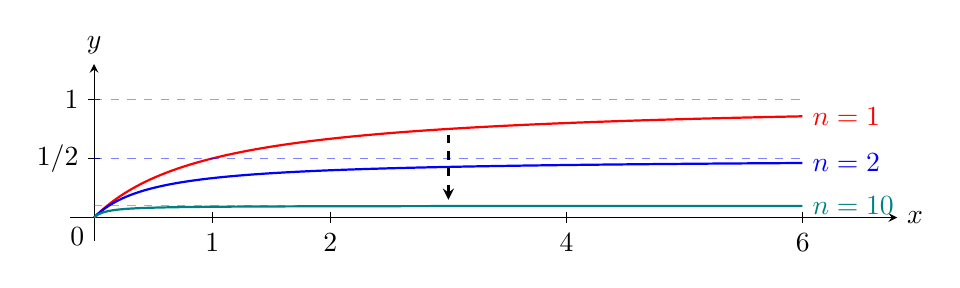
\begin{tikzpicture}[scale=1.5, >=stealth]
            \def\xmax{6}
            \def\ymax{1.3}

            \draw[->] (-0.2, 0) -- (\xmax+0.8, 0) node[right] {$x$};
            \draw[->] (0, -0.2) -- (0, \ymax) node[above] {$y$};

            \draw (1, 0.05) -- (1, -0.05) node[below] {$1$};
            \draw (2, 0.05) -- (2, -0.05) node[below] {$2$};
            \draw (4, 0.05) -- (4, -0.05) node[below] {$4$};
            \draw (6, 0.05) -- (6, -0.05) node[below] {$6$};
            
            \draw (0.05, 1) -- (-0.05, 1) node[left] {$1$};
            \draw (0.05, 0.5) -- (-0.05, 0.5) node[left] {$1/2$};
            \node[below left] at (0,0) {$0$};

            \draw[red, dashed, thin, opacity=0.5] (0, 1) -- (\xmax, 1);
            \draw[red, thick, domain=0:\xmax, samples=200] plot (\x, {\x / (1 + \x)});
            \node[red, right] at (\xmax, {\xmax / (1 + \xmax)}) {$n=1$};

            \draw[blue, dashed, thin, opacity=0.5] (0, 0.5) -- (\xmax, 0.5);
            \draw[blue, thick, domain=0:\xmax, samples=200] plot (\x, {\x / (1 + 2*\x)});
            \node[blue, right] at (\xmax, {\xmax / (1 + 2*\xmax)}) {$n=2$};

            \draw[teal, dashed, thin, opacity=0.5] (0, 0.1) -- (\xmax, 0.1);
            \draw[teal, thick, domain=0:\xmax, samples=200] plot (\x, {\x / (1 + 10*\x)});
            \node[teal, right] at (\xmax, {\xmax / (1 + 10*\xmax)}) {$n=10$};

            \draw[->, black, thick, dashed] (3, 0.7) -- (3, 0.15);
        \end{tikzpicture}
    \end{center}
}

In generale per la convergenza uniforme, vogliamo che \(|f_n(x) - f(x)| < \varepsilon\),
cioè \(f(x) - \varepsilon < f_n(x) - f(x) + \varepsilon\).
In altre parole, vogliamo che i grafici delle \(f_n\) siano definitivamente contenuti
nella regione delimitata dalle curve \(f-\varepsilon\) e \(f + \varepsilon\).

Per esempio, nel secondo esempio sopra,
\begin{align*}
    |f_n(x) - f(x)| = \frac12
\end{align*}
per tutte le \(x \in S\) e \(n \in \naturalnumbers\), quindi non vi è convergenza uniforme.

\end{document}